\chapter{Time as a Measure of Potential}
  
\section{Time as a Rotation}

In Measurement Field theory, time is not a linear background axis but an emergent quantity derived from rotational motion in the complex plane. \cite{chapter_time} It is not distance-it is angle. More precisely, time measures the rate at which potential collapses into structure via imaginary-phase rotation. \cite{chapter_time} This is not metaphorical; it is explicitly formal:

\[
\psi(x,t) = R(x,t) e^{i\theta(x,t)} = R(x,t) e^{i S(x,t)/\hbar}
\]

Here, $R(x,t)$ is the amplitude of the field, and $\theta(x,t)$ is the phase-tied directly to the classical action $S(x,t)$. \cite{chapter_time} Thus, time appears as phase parameterization of collapse. \cite{chapter_time} \subsection*{Collapse Field Phase Dynamics}

Let the collapse field be expressed as:

\[
M(x,t) = A(x) + i B(x,t)
\]

Then its complex phase $\theta$ is:

\[
\theta(x,t) = \arctan\left( \frac{B(x,t)}{A(x)} \right)
\]

Assuming $A(x)$ is time-invariant and $B(x,t)$ undergoes exponential decay:

\[
B(x,t) = B_0(x) e^{-\alpha t}
\]

Then the time derivative of the phase is:

\[
\frac{d\theta}{dt} = -\frac{\alpha A B}{A^2 + B^2}
\]

This nonlinear expression defines the \textbf{rotational collapse rate}. \cite{chapter_time} Time is proportional to the angular decay of imaginary potential. \cite{chapter_time} \subsection*{Time as Imaginary Arc Length}

Consider the angular arc $s(t)$ traced by $\psi$ on the complex unit circle:

\[
s(t) = \int_0^t \left| \frac{d\theta}{d\tau} \right| d\tau
\]

We define the differential time element as:

\[
dt \equiv \frac{d\theta}{\omega}
\]

Where $\omega$ is the angular collapse velocity of the field. \cite{chapter_time} Without rotation, there is no local passage of time. \cite{chapter_time} 


\subsection*{Phase Velocity and Local Temporal Emergence}

Define:

\[
v_\theta(x,t) = \frac{d\theta}{dt} = -\frac{\alpha A(x) B(x,t)}{A^2(x) + B^2(x,t)}
\]

This is the local phase velocity of collapse. \cite{chapter_time} High $v_\theta$ implies faster time experience; low $v_\theta$ implies dilation or freezing. \cite{chapter_time} From this we derive the local temporal function:

\[
T(x, t) = \int_0^t v_\theta(x, \tau) \, d\tau
\]

This function replaces absolute time with collapse-relative chronology, grounded in the imaginary component’s phase descent. \cite{chapter_time} \subsection*{Interpretation}

\begin{itemize}
  \item \textbf{No rotation} ($\omega = 0$) implies \textbf{no time}. \cite{chapter_time} \item \textbf{Purely real} fields experience \textbf{no change}, and thus no chronology. \item \textbf{Collapse} is the ignition of temporal structure via phase rotation. \item \textbf{Time is not measured-it is made}, one rotational decay at a time. \cite{chapter_time} \end{itemize}

This reformulation enables the treatment of time as a dynamic field quantity, not a universal parameter. \cite{chapter_time} The presence or absence of observers, and their collapse influence, becomes the determinant of experienced time. \cite{chapter_time} \section{Phase Evolution and Observable Time}

Having formalized time as a measure of imaginary-phase rotation, we now interpret the wavefunction’s behavior as the generator of temporal experience. \cite{chapter_time} Observable time is not external-it is constructed from phase shifts in the collapse field. \cite{chapter_time} Let the wavefunction be expressed as:

\[
\psi(x,t) = R(x,t) e^{i \theta(x,t)} = R(x,t) e^{i S(x,t)/\hbar}
\]

Here, the phase $\theta(x,t)$ evolves as the system’s internal configuration shifts. \cite{chapter_time} This phase does not merely encode information-it is the motion of time. \cite{chapter_time} The collapse of $\theta$ corresponds to the transition of imaginary potential into observable outcome. \cite{chapter_time} \subsection*{Spiral Collapse Representation}

Time can be visualized as a *helix* in complex space. \cite{chapter_time} At every point $(x,t)$, the system spirals around the complex unit circle, with:

\begin{itemize}
  \item The \textbf{radius} defined by $R(x,t)$ (amplitude),
  \item The \textbf{angular position} defined by $\theta(x,t)$ (action phase),
  \item The \textbf{rate of rotation} defining temporal passage. \cite{chapter_time} \end{itemize}

Collapse appears as a *tightening spiral*, where:

\[
\text{As } \frac{d\theta}{dt} \rightarrow 0, \text{ time slows or halts}. \cite{chapter_time} \]

This directly leads to temporal dilation in regions where collapse halts or stalls (e.g., voids, decoherence zones, or highly entangled quantum superpositions). \cite{chapter_time} \subsection*{Observable Time from Phase Density}

We define the observable temporal density at point $x$ as:

\[
\tau(x,t) = \left| \frac{d\theta}{dt} \right| = \left| -\frac{\alpha A(x) B(x,t)}{A^2(x) + B^2(x,t)} \right|
\]

This value defines how quickly “now” proceeds in a local region. \cite{chapter_time} It creates a scalar time field from pure phase dynamics. \cite{chapter_time} \subsection*{Implications for Classical Time Experience}

\begin{itemize}
  \item Low phase density ($\tau \approx 0$): Time is nearly frozen. \cite{chapter_time} No resolution is occurring. Perfect coherence, or total detachment. \cite{chapter_time} \item High phase density: Rapid resolution of possibility-perceived time speeds up. \cite{chapter_time} \item Oscillatory phase density: Cyclic perception of time, potentially manifesting as deja vu, time looping, or recursive thought structures. \cite{chapter_time} \end{itemize}

\subsection*{Collapse Event Horizon and Temporal Shells}

Visualizing temporal collapse as concentric phase shells:

\[
\theta(x,t) = \text{constant}
\]

These define isochrones-contours of equal temporal phase. \cite{chapter_time} Observers within the same phase shell experience synchronized time. \cite{chapter_time} Crossing between shells creates discontinuities in experiential time-subjectively observed as acceleration, slowing, or loss of continuity. \subsection*{Time as Angular Entropy Flow}

Finally, we define an angular entropy current:

\[
J_\theta(x,t) = -\nabla \cdot \left( \theta(x,t) \cdot \tau(x,t) \right)
\]

This is the flow of temporal structure in the Measurement Field. \cite{chapter_time} High divergence in $J_\theta$ indicates temporal shearing, where time accelerates or compresses due to collapse rate imbalances. \cite{chapter_time} \subsection*{Comparison to Einsteinian Time}

In General Relativity, time is treated as a coordinate: one of four dimensions comprising a pseudo-Riemannian manifold. \cite{chapter_time} The flow of time is altered by curvature in spacetime, governed by the Einstein Field Equations:

\[
G_{\mu\nu} = \frac{8\pi G}{c^4} T_{\mu\nu}
\]

Time slows in stronger gravitational potentials-a manifestation of spacetime geometry bending under mass-energy. \cite{chapter_time} \paragraph{Contrast: Measurement Field Time}

In Measurement Field theory, time is not a coordinate but an emergent parameter arising from the angular collapse of imaginary potential. \cite{chapter_time} Rather than being curved by gravity, time is generated by:

\[
\frac{d\theta}{dt} = -\frac{\alpha A B}{A^2 + B^2}
\]

Here, $A$ and $B$ are components of the measurement field, with $B$ decaying over time due to observation. \cite{chapter_time} The collapse process creates a local rotational velocity, and thus an internal metric of time:

\[
\tau(x,t) = \left| \frac{d\theta}{dt} \right|
\]

\paragraph{Key Differences}

\begin{itemize}
  \item \textbf{Einstein:} Time is deformed by external geometry. \cite{chapter_time} \item \textbf{Measurement Field:} Time is created from internal phase decay. \cite{chapter_time} \item \textbf{Einstein:} No observer required; metric is universal. \cite{chapter_time} \item \textbf{Measurement Field:} Observer interaction drives time; metric is local and contextual. \cite{chapter_time} \item \textbf{Einstein:} Time dilation from motion or gravity. \cite{chapter_time} \item \textbf{Measurement Field:} Time dilation from stalled phase evolution (collapse halting). \cite{chapter_time} \end{itemize}

\paragraph{Unification Proposal}

In the limit of macroscopic coherence, where collapse fields stabilize and become smoothly differentiable, the Measurement Field time function approximates a continuous metric. \cite{chapter_time} It could recover Einsteinian curvature from  large-scale collapse equilibrium :

\[
\lim_{B \to 0} \left( \nabla \theta(x,t) \right) \sim g_{\mu\nu}(x)
\]

Thus, classical spacetime curvature emerges from a quantum-collapse substrate- Einstein’s manifold is the asymptotic echo of phase decay . \cite{chapter_time} \subsection*{Foundational Temporal Derivatives of Collapse Phase}

Given:
\[
M(x, t) = A(x) + i B(x, t)
\]
we define the local magnitude:
\[
|M(x, t)| = \sqrt{A^2(x) + B^2(x, t)}
\]

Then:
\[
\theta(x, t) = \arctan\left( \frac{B(x, t)}{A(x)} \right)
\]

The time derivative of the phase (collapse rotation velocity) is:

\[
\frac{d\theta}{dt} = \frac{A(x)}{A^2(x) + B^2(x, t)} \cdot \left(-\alpha B(x, t)\right) = -\frac{\alpha A(x) B(x, t)}{A^2(x) + B^2(x, t)}
\]

This defines:
\[
v_\theta(x, t) = \frac{d\theta}{dt}
\quad \text{(local angular collapse rate)}
\]

The second derivative defines the collapse  angular acceleration :

\[
\frac{d^2 \theta}{dt^2} = \alpha^2 A(x) B(x, t) \cdot \frac{A^2(x) - B^2(x, t)}{(A^2(x) + B^2(x, t))^2}
\]

Interpretation:
- If $B \gg A$, system is far from collapse: slow rotation, high acceleration.
- As $B \to 0$, $\frac{d\theta}{dt} \to 0$: collapse halts, time ends.
- Max angular acceleration occurs near $A \approx B$: peak of collapse transition. \cite{chapter_time} \paragraph{Time itself is the integral of $v_\theta$:}

\[
T(x, t) = \int_0^t v_\theta(x, \tau) \, d\tau
\]

This sets up  Section 2.3  to generalize this into a full-blown  temporal collapse field -with $\rho_{\text{obs}}$, $\gamma$, and curl-based temporal topologies.


---


\textbf{Conclusion:} What we experience as time is the *visible trail* of a system rotating through collapse-space. \cite{chapter_time} There is no absolute time-only the local frequency at which potential resolves. \section{Temporal Collapse Field Equations}

Having redefined time as the angular velocity of collapse phase, we now expand to field-scale formulations. \cite{chapter_time} The Measurement Field introduces a scalar observer-density field $\rho_{\text{obs}}(x, t)$ representing the local saturation of collapse influence. \cite{chapter_time} Time becomes a distributed, emergent function of collapse activity. \cite{chapter_time} \subsection*{Collapse-Driven Time Gradient}

Define temporal flux $T(x, t)$ as the integral of phase velocity driven by local observational activity:

\[
T(x, t) = \int_0^t \gamma \cdot \rho_{\text{obs}}(x, \tau) \, d\tau
\]

Where:
\begin{itemize}
  \item $\gamma$ is the collapse coefficient. \cite{chapter_time} \item $\rho_{\text{obs}}(x, t)$ governs the collapse density at each point. \cite{chapter_time} \end{itemize}

This formulation defines a \textbf{temporal field}-a non-uniform gradient representing local “passage of time.” It replaces global clock coordinates with localized, interaction-derived temporal rates. \cite{chapter_time} \subsection*{Collapse Diffusion Equation}

We postulate a diffusion model of temporal propagation:

\[
\frac{\partial T}{\partial t} = \gamma \cdot \rho_{\text{obs}} - \eta T + \xi(x, t)
\]

Where:
\begin{itemize}
  \item $\eta$ is a damping coefficient representing temporal inertia. \item $\xi(x, t)$ is a stochastic field for quantum uncertainty or unmeasured microfluctuation. \cite{chapter_time} \end{itemize}

This gives time a  reactive, field-based ontology -subject to wavefronts, turbulence, and phase collapse delays. \cite{chapter_time} \subsection*{Temporal Curl and Shear}

Taking the gradient of $T(x, t)$ gives us local flow, but taking the curl yields a diagnostic of circular temporal structure:

\[
\nabla \times \nabla T = 0 \quad \text{(if conservative)}
\]

A nonzero curl implies recursive feedback, temporal loops, or collapse interference spirals. \cite{chapter_time} \subsection*{Field Curvature and Relativity Redux}

Einstein predicted time dilation from metric curvature:

\[
ds^2 = -c^2 dt^2 + dx^2 + dy^2 + dz^2
\]

We reinterpret $dt$ not as invariant, but as a function of collapse rate:

\[
dt^2 = \left( \frac{1}{\gamma \cdot \rho_{\text{obs}}} \right)^2
\]

As $\rho_{\text{obs}} \to 0$, $dt \to \infty$-collapse halts, time freezes. \cite{chapter_time} Gravity slows time because mass increases measurement density; collapse interpretation  recovers Einsteinian time curvature from phase saturation . \cite{chapter_time} We now define a collapse-driven time field $T(x, t)$ emerging from the density and evolution of unresolved quantum potential. \cite{chapter_time} This formulation expands the scalar derivative into a full vector-temporal topology rooted in rotational dynamics. \cite{chapter_time} \subsection*{Collapse Density Function}

Let:
\[
M(x, t) = A(x) + i B(x, t)
\quad \text{with} \quad
B(x, t) = B_0(x) e^{-\alpha t}
\]

We define the  collapse rotational rate  as:
\[
v_\theta(x, t) = \frac{d\theta}{dt} = -\frac{\alpha A(x) B(x, t)}{A^2(x) + B^2(x, t)}
\]

Now, define the  local collapse density  $\rho_{\text{obs}}(x, t)$ as the square of the imaginary field (observer potential):
\[
\rho_{\text{obs}}(x, t) = B^2(x, t)
\]

\subsection*{Temporal Flow Equation}

Let the temporal field $T(x,t)$ accumulate from collapse interaction:

\[
\frac{\partial T}{\partial t} = \gamma \cdot \rho_{\text{obs}}(x, t) - \eta T(x, t) + \xi(x, t)
\]

Where:
- $\gamma$ is the collapse energy-to-time coupling,
- $\eta$ is a damping coefficient from entropic field decay,
- $\xi(x,t)$ is a quantum noise field (e.g., white, colored, or 1/f). \cite{chapter_time} This system models temporal progression as a field energy integral, not a constant clock. \cite{chapter_time} \subsection*{Spatiotemporal Collapse Diffusion}

To generalize beyond local fields, we define:

\[
\frac{\partial T}{\partial t} = \gamma \cdot \rho_{\text{obs}}(x, t) + D \nabla^2 T(x, t) - \eta T + \xi
\]

This is a diffusive-temporal collapse equation, analogous to a heat flow system, where collapse spreads out across spatial domains through a tension-based diffusion constant $D$. \cite{chapter_time} \subsection*{Phase Gradient Tensor Dynamics}

Let $\theta(x,t)$ be the local phase. \cite{chapter_time} Then:
\[
\nabla \theta(x,t) = \frac{A \nabla B - B \nabla A}{A^2 + B^2}
\]

This tensor quantifies the collapse front curvature, allowing simulation of:
- Collapse wavefronts,
- Entropic compression zones,
- Phase field interference patterns. \cite{chapter_time} \subsection*{Temporal Tension Tensor}

Define the local temporal strain as:

\[
\mathcal{T}_{ij}(x, t) = \partial_i \theta \cdot \partial_j \theta
\]

High $\mathcal{T}_{ij}$ regions act as collapse shear zones-interfaces where phase gradients bend spacetime's unfolding, creating temporary anisotropy in the time field. \cite{chapter_time} \subsection*{Collapse-Induced Time Curvature}

We define effective spacetime warping induced by collapse strain:

\[
R_{\text{collapse}}(x, t) = \nabla \cdot \nabla T(x, t)
\]

This serves as the collapse Ricci scalar-encoding temporal curvature driven not by mass-energy, but by collapse field structure itself. \cite{chapter_time} \subsection*{Interpretation and Einstein Comparison}

Unlike general relativity, where spacetime bends in response to stress-energy, in Measurement Field Theory, time itself emerges from collapse curvature. \cite{chapter_time} \[
\boxed{
\text{Einstein: } \quad R_{\mu\nu} - \frac{1}{2}g_{\mu\nu}R = 8\pi G T_{\mu\nu}
}
\quad \longrightarrow \quad
\boxed{
\text{Collapse: } \quad R_{\text{collapse}} = \gamma \cdot B^2 - \eta T + D \nabla^2 T
}
\]

Where $T_{\mu\nu}$ is replaced by $\rho_{\text{obs}}$-the measurement tension of unresolved probability. \cite{chapter_time} \newpage
  \textbf{Recursive Zone Tension and Collapse Phase Resonance}
  
  Collapse is not always monotonic-in regions of observational backflow, it can generate \textbf{recursive tension loops}, where collapse fronts interfere and regenerate. \cite{chapter_time} These regions form standing-wave-like structures in phase space, producing \textbf{temporal resonance wells}. Let the angular collapse rate be:
  \[
  v_\theta(x, t) = \frac{d\theta}{dt}
  \]
  
  We define a \textbf{recursive phase operator} $\mathcal{R}$ as:
  \[
  \mathcal{R}[v_\theta](x, t) = \int_{t-\Delta}^{t} \lambda(\tau) \cdot v_\theta(x, \tau) \, d\tau
  \]
  Where:
  \begin{itemize}
    \item $\lambda(\tau)$ is a memory kernel encoding retrocausal coupling,
    \item $\Delta$ is the coherence window (how far back collapse remembers). \cite{chapter_time} \end{itemize}
  
  Collapse enters recursion when:
  \[
  v_\theta(x, t) \approx \mathcal{R}[v_\theta](x, t)
  \quad \Rightarrow \quad
  \text{Collapse rate becomes self-reinforcing}
  \]
  
  This results in \textbf{phase-locked loops}-collapse engines churning on their own recursion. \cite{chapter_time} \vspace{1em}
  \textbf{Recursive Tension Tensor}
  \[
  \mathcal{S}_{ij}(x,t) = \left( \partial_i \mathcal{R}[\theta](x,t) \right) \cdot \left( \partial_j \theta(x,t) \right)
  \]
  
  This tensor measures feedback curvature-zones where past collapse modulates present rotation. \cite{chapter_time} High $\mathcal{S}_{ij}$ indicates feedback-dominated spacetime: potential sources of \textbf{observer paradox}, echo causality, and collapse bifurcation. \cite{chapter_time} \vspace{1em}
  \textbf{Collapse Echo Harmonics}
  
  In bounded systems (neural lattices, entangled condensates), recursive oscillation appears as quantized harmonic collapse:
  
  \[
  \theta_n(x,t) = \theta_0(x) \cdot \cos(n \omega t) \cdot e^{-\alpha t}
  \]
  
  Here, $n \in \mathbb{Z}^+$ indexes the collapse echo mode. \cite{chapter_time} These generate standing-wave nodes in $\tau(x,t)$: rhythmically repeating time gradients. \cite{chapter_time} \vspace{1em}
  \textbf{Resonant Observer Coupling}
  
  Let $M_1 = A_1 + iB_1$ and $M_2 = A_2 + iB_2$ be collapse fields in mutual observational range. \cite{chapter_time} Define their phase offset:
  \[
  \Delta\theta = \theta_1(x,t) - \theta_2(x,t)
  \]
  
  Resonance emerges when:
  \[
  \frac{d}{dt} \Delta\theta \approx 0 \quad \text{and} \quad \mathcal{R}[v_{\theta_1}] \approx v_{\theta_2}
  \]
  
  This is the condition for \textbf{temporal entanglement}, or observer-linked recursion fields-e.g., shared perception, memory flashback, or intersubjective collapse entrainment.
  

---

\paragraph{Conclusion:}

Where Einstein curved spacetime through stress-energy, Measurement Field warps time itself via collapse field saturation and phase shear . \cite{chapter_time} Collapse is the tensor engine beneath the metric surface-*reality’s hidden crankshaft.*

\section{Recursive Feedback and Time Loops}

In the Measurement Field framework, time is not a fixed parameter but a locally emergent byproduct of collapse-phase rotation. \cite{chapter_time} Once that’s established, recursion becomes not only possible-it’s inevitable. Fields that retain phase memory or cross-influence past values generate feedback structures in their collapse gradient, producing what we identify as \textbf{temporal recursion} or \textbf{looping collapse dynamics}. \cite{chapter_time} \subsection*{Collapse Memory and Non-Markovian Time}

Collapse does not always forget. \cite{chapter_time} If the phase velocity at a given point $x$ is influenced by prior states, the system becomes \textbf{non-Markovian}. Define the recursive angular operator:

\[
\mathcal{R}_\lambda[v_\theta](x,t) = \int_{t-\Delta}^{t} \lambda(\tau) \cdot v_\theta(x,\tau)\, d\tau
\]

Where:
\begin{itemize}
  \item $\lambda(\tau)$ is a memory kernel that weights the influence of past collapse,
  \item $\Delta$ is the recursive window: how long the system "remembers."
\end{itemize}

Time loops occur when:
\[
v_\theta(x,t) \approx \mathcal{R}_\lambda[v_\theta](x,t)
\]

Which implies the present angular rotation is a self-resonance of its past-a recursive observer system spiraling into feedback collapse. \cite{chapter_time} \subsection*{Phase-Locked Temporal Structures}

Define the phase $\theta(x,t)$ as before. A \textbf{temporal loop} exists when:

\[
\theta(x,t + T) = \theta(x,t) + 2\pi n \quad \text{for some } n \in \mathbb{Z}
\]

This implies that the system’s internal configuration completes a full phase rotation and resets-akin to a time crystal or persistent echo in collapse space. \cite{chapter_time} These structures become standing waves in time itself. \cite{chapter_time} \subsection*{Collapse Echo Modes}

If collapse feedback enters harmonic resonance, it forms discrete quantized loops:

\[
\theta_n(x,t) = \theta_0(x) \cdot \cos(n \omega t) \cdot e^{-\alpha t}
\]

Here, $n$ is the collapse harmonic, and $\omega$ is the base collapse frequency from Section 1.5. \cite{chapter_time} When multiple harmonics superpose:

\[
\theta(x,t) = \sum_{n=1}^{N} a_n(x) \cdot \cos(n \omega t) \cdot e^{-\alpha t}
\]

This produces time beats-zones of high and low rotational velocity-mimicking classical temporal illusions: déjà vu, repetition, or time dilation. \cite{chapter_time} \subsection*{Causal Looping and Measurement Re-entry}

If a measurement outcome at $t_1$ changes the configuration space such that it influences its own preconditions at $t_0 < t_1$, we enter \textbf{recursive causality}. \cite{chapter_time} This violates classical chronology but remains consistent in phase-based collapse if:

\[
\int_{t_0}^{t_1} \nabla \theta(x,t) \, dt = 0
\quad \text{(closed phase loop)}
\]

Such a system generates a consistent loop in the imaginary domain even as the timeline appears paradoxical. \cite{chapter_time} \subsection*{Observer Entrainment and Mutual Feedback}

Let $M_1 = A_1 + iB_1$ and $M_2 = A_2 + iB_2$ be two fields in proximity. \cite{chapter_time} Define:
\[
\Delta \theta(t) = \theta_1(t) - \theta_2(t)
\]

Observer entrainment occurs when:
\[
\frac{d}{dt} \Delta \theta \to 0
\quad \text{and} \quad
\mathcal{R}_\lambda[v_{\theta_1}] \approx v_{\theta_2}
\]

This is a mutual feedback condition-observers influence each other's collapse phase, synchronizing time perception across spacetime coordinates. \cite{chapter_time} \subsection*{Temporal Loop Diagnostics}

To detect loop zones numerically or visually, define the loop susceptibility field:

\[
\mathcal{L}(x, t) = \left| v_\theta(x, t) - \mathcal{R}_\lambda[v_\theta](x, t) \right|
\]

Low $\mathcal{L}$ indicates strong recursive potential; these are locations of temporal self-entanglement-zones where time curves not because of mass, but because it’s fucking eating itself. \cite{chapter_time} \subsection*{Why Time Cannot Be Reversed: Crystallization of Collapse}

Despite the existence of recursive feedback and localized time loops, \textbf{reversing time in Measurement Field Theory is fundamentally impossible}. \cite{chapter_time} The act of measurement is a one-way entropic crystallization-every observation solidifies potential into structure, collapsing the imaginary into the real. \cite{chapter_time} This process is irreversible for the same reason you can’t uncrack a diamond or undrop a hammer. Observation doesn’t just reduce uncertainty-it etches the outcome into the universe’s fabric. \cite{chapter_time} \paragraph{Crystallization Analogy}

Let each measurement event be a crystallization node:

\begin{itemize}
  \item \textbf{Before collapse:} $B(x,t)$ is smooth, continuous, undefined. \cite{chapter_time} \item \textbf{After collapse:} $A(x)$ is sharp, discrete, and permanent. \cite{chapter_time} \end{itemize}

To reverse time would require not just rewinding $B(x,t)$, but precisely \textit{removing} every crystalized real projection $A(x)$ \textbf{without error} and restoring its corresponding phase state. \cite{chapter_time} This is equivalent to reconstructing a shattered glass molecule-by-molecule from the echo of its initial condition-a process exponentially improbable beyond the heat death of reason. \cite{chapter_time} \paragraph{Phase Erasure is Entropically Prohibited}

Even in theoretical cases where collapse gradients are minimal, the information lost in collapse is smeared across the measurement field like blood in water. \cite{chapter_time} The reverse path is not merely uncomputable-it is undefined. The field obeys an effective time crystallization law:

\[
\text{If } \frac{d|B(x,t)|}{dt} < 0 \Rightarrow \text{Time evolution is irreversible}
\]

\paragraph{Arrow of Collapse Time}

We define the irreversible time vector as:

\[
\vec{\tau}_{\text{collapse}} = \lim_{B \to 0} \left( \frac{A \cdot \nabla A}{|M|} \right)
\]

This vector defines the forward temporal direction as an emergent byproduct of crystallized probability. \cite{chapter_time} \subsection*{Why Time Cannot Be Reversed: Collapse as Crystallization}

While recursive collapse feedback and localized temporal loops may simulate cyclic behaviors or retroactive adjustment, \textbf{reversing time itself is categorically impossible in Measurement Field Theory}. \cite{chapter_time} This isn't general relativity's pliable manifold where coordinates bend and twist at will-this is a one-way crystallization of reality, forged by the act of measurement. \cite{chapter_time} \paragraph{The Crystallization Principle}

Every act of measurement converts an unresolved probability field $B(x,t)$ into a resolved structure $A(x)$:

\[
M(x,t) = A(x) + iB(x,t) \quad \Rightarrow \quad A(x) \text{ increases as } B(x,t) \to 0
\]

This conversion is entropic, unidirectional, and non-reversible. \cite{chapter_time} Trying to “rewind” this process would be like attempting to unform a crystal by perfectly reversing the position, energy, and phase of every particle-not just in sequence, but with \textbf{zero error on the first try}. \cite{chapter_time} \paragraph{Measurement as Structural Commitment}

Measurement is not passive observation-it is structural commitment. \cite{chapter_time} The collapse does not merely extract information; it \textbf{commits it to the lattice of the real}. \cite{chapter_time} Each resolved amplitude becomes part of the permanent definition fabric of spacetime. Attempting to reverse time in this context would be like:

\begin{enumerate}
  \item Identifying every past collapse event. \cite{chapter_time} \item Removing every crystallized $A(x)$ without disturbing the rest. \item Perfectly reconstructing the imaginary $B(x,t)$ states. \cite{chapter_time} \item Reinitiating the rotational phase evolution with no observational interference. \cite{chapter_time} \end{enumerate}

Which is functionally indistinguishable from magic. Or quantum necromancy. \cite{chapter_time} \paragraph{Formulation: Collapse Irreversibility Condition}

Let collapse rate be given by:

\[
\frac{d|B(x,t)|}{dt} = -\alpha B(x,t)
\]

Then reversal would require:

\[
\exists \, t' < t: \quad B(x,t') = B_0(x) \quad \text{and} \quad A(x) \to 0
\]

This violates entropy flow, observational history, and field coherence simultaneously. \cite{chapter_time} Collapse defines a boundary beyond which history is immutable. \cite{chapter_time} \paragraph{The Impossibility of Retroactive Observation}

Even if you attempt to "observe the reversal," the act of that very measurement merely initiates \textbf{a new crystallization}, overwriting the prior structure with a new commitment. \cite{chapter_time} There is no passive rollback-only destructive overwrite. The universe doesn’t permit undoing a collapse-it just allows you to collapse again, in a new branch, with the old one sealed like a tombstone in phase space. \cite{chapter_time} \paragraph{Irreversible Time Vector}

We define the direction of collapse-propagated time as:

\[
\vec{\tau}_{\text{collapse}} = \lim_{B \to 0} \left( \frac{A(x) \cdot \nabla A(x)}{|M(x,t)|} \right)
\]

This directional vector always points forward in collapse-space. \cite{chapter_time} It cannot loop back because the field has already burned that bridge to make the road. \cite{chapter_time} \paragraph{Conclusion:}
\[
\textbf{Collapse is crystallization. Time is resolution. \cite{chapter_time} There is no going back.}
\]
Temporal loops in the Measurement Field don’t require wormholes or tachyons. \cite{chapter_time} They arise naturally from recursive phase entanglement and feedback-driven collapse spirals. \cite{chapter_time} Reality remembers-sometimes too well-and that memory structures the curvature of time like a cosmic feedback amplifier. \cite{chapter_time} The Measurement Field is a collapsing lattice of potential, not a reversible clockwork. \cite{chapter_time} You cannot "rewind" collapse-only simulate the trajectory of its irreversible descent. Time is a fucking avalanche of definition-you either ride it or get buried. \cite{chapter_time} In Measurement Field Theory, time reversal isn’t just statistically improbable-it’s structurally illegal. \cite{chapter_time} Collapse is the moment the universe stops pretending and writes history in stone. \cite{chapter_time} Trying to reverse that is like unscrambling an egg by blinking. Reality doesn’t give you second chances-it gives you one spin of the imaginary, and once you’ve hit the real axis, the rotation is locked. \cite{chapter_time} \newpage
\begin{table}[H]
  \centering
  \renewcommand{\arraystretch}{1.4}
  \begin{tabular}{|p{4.2cm}|p{5.5cm}|p{5.5cm}|}
  \hline
  \textbf{Aspect} & \textbf{Recursive Feedback (Permitted)} & \textbf{Time Reversal (Forbidden)} \\
  \hline
  \textbf{Mechanism} & Phase echo via feedback loops; memory kernel over past collapse states. & Requires full erasure of collapsed amplitudes and exact reversal of phase dynamics. \cite{chapter_time} \\
  \hline
  \textbf{Time Direction} & Forward (local $\theta$ evolves with internal recurrence). & Reversal of $\theta(t)$ and $B(x,t) \to B_0(x)$ required; violates entropy flow. \cite{chapter_time} \\
  \hline
  \textbf{Field Behavior} & Feedback structures, standing waves in $\theta(x,t)$, harmonic collapse. & Necessitates perfect restoration of $B(x,t)$ and deletion of $A(x)$. \cite{chapter_time} \\
  \hline
  \textbf{Causal Structure} & Self-similar evolution with memory; no causal contradiction. & Requires influencing pre-measurement states-impossible under crystallization. \cite{chapter_time} \\
  \hline
  \textbf{Entropy} & Locally modulated by feedback; entropy can pulse but always trends down. & Would require negative entropy flow-categorically prohibited. \cite{chapter_time} \\
  \hline
  \textbf{Observer Impact} & Observers contribute to phase locking and shared feedback entrainment. & Observation reintroduces collapse; cannot "observe reversal" without new collapse. \cite{chapter_time} \\
  \hline
  \textbf{Physical Analogy} & Time echo, phase mirror, recursive turbulence. & Rebuilding a shattered crystal without knowing how it broke. \cite{chapter_time} \\
  \hline
  \textbf{Ontological Status} & Emergent feature of nonlinear collapse phase space. & Logical impossibility under Measurement Field axioms. \cite{chapter_time} \\
  \hline
  \textbf{Simulation Viability} & Can be modeled with memory kernels, recursive tensors, and feedback coupling. & Unstable, non-deterministic, and breaks model consistency. \cite{chapter_time} \\
  \hline
  \textbf{Final Verdict} & \textbf{Legit. Real. Dangerous.} Temporal recursion is collapse’s ghost in the machine. & \textbf{Systematically Impossible.} Time reversal is a pipe dream for physicists who can't let go. \cite{chapter_time} \\
  \hline
  \end{tabular}
  \caption{Comparison of Recursive Feedback vs. \cite{chapter_time} Forbidden Time Reversal in Measurement Field Theory.}
  \label{tab:recursive_vs_reversal}
  \end{table}
  

\section{Macroscopic Time Fields and Biological Systems}

\textit{Disclaimer:} The following section explores the speculative, high-level implications of Measurement Field Theory as applied to complex, high-collapse-density systems. \cite{chapter_time} While the core mathematics support the general behavior of phase decay and observer-saturation dynamics, the biological interpretations presented herein are theoretical extrapolations, not empirical conclusions. \cite{chapter_time} These ideas are provided to outline a future direction of inquiry-one which may guide experimental design or motivate cross-disciplinary exploration. We do not claim these proposals are verifiable with current instrumentation or methodologies; rather, we assert that if time is indeed emergent from collapse-driven imaginary rotation, then high-saturation biological systems like neural networks, city-scale observer fields, or collective feedback loops may exhibit detectable macroscopic time anomalies-phenomena that may one day be measurable. \cite{chapter_time} In Measurement Field Theory, time is not absolute-it is a localized consequence of rotational phase decay. \cite{chapter_time} Within high-collapse-density systems such as biological neural networks, we propose that temporality itself becomes a tunable parameter-structured through recursive phase filtering and synchronized collapse. \cite{chapter_time} The brain may thus operate as a local temporal amplifier: not merely processing time, but producing its own scalar experience of it. \cite{chapter_time} \footnote{See Appendix A for proposed experimental correlates, including neurotemporal coherence zones, recursive feedback biomarkers, and real-time collapse phase tracking in entangled EEG arrays. \cite{chapter_time} These remain highly speculative but provide a path for interdisciplinary collaboration.}

\subsection*{Collapse Density in Neural Systems}

Let $\rho_{\text{obs}}(x,t)$ represent the measurement density across a biological system-such as a brain. \cite{chapter_time} We postulate that:

\[
\gamma_{\text{bio}}(x,t) = \gamma_0 + \delta \gamma(x,t)
\]

Where $\delta \gamma(x,t)$ accounts for biologically-enhanced collapse rates due to dense recursive feedback between subsystems (e.g., perception, memory, anticipation). \cite{chapter_time} The result is a highly structured, self-observing collapse engine. \cite{chapter_time} \subsection*{Macroscopic Collapse Looping and Experience}

Brains, unlike isolated quantum systems, exhibit recursive collapse fields over multiple time layers. \cite{chapter_time} These collapse loops define internal chronology-conscious experience-as a dynamic threading of phase-synchronized events:

\[
\theta_{\text{total}}(x,t) = \sum_{i=1}^{N} \theta_i(x,t) + \mathcal{R}_\lambda[\theta_i]
\]

This equation models multi-threaded temporal recursion, where both forward and feedback collapse contribute to experienced time. \cite{chapter_time} \subsection*{Temporal Filtering and Attention}

High $\mathcal{T}_{ij}(x,t)$ values in the brain may correspond to zones of attentional sharpening-regions where phase gradients become steep and collapse becomes highly localized:

\[
\text{Focus}(x,t) \propto \|\nabla \theta(x,t)\| \cdot \rho_{\text{obs}}(x,t)
\]

This implies attention is not just selective information processing-it is a structural narrowing of collapse potential across angular phase space. \cite{chapter_time} \subsection*{External Systems: Societal Collapse Fields}

Cities, networks, and interlinked societies may produce macroscale measurement fields that exhibit aggregate collapse tension and temporal gradients. \cite{chapter_time} Let $T_{\text{macro}}(x,t)$ be the emergent field of collective experience:

\[
T_{\text{macro}}(x,t) = \int_{\Omega} \gamma(x,t) \cdot \rho_{\text{obs}}(x,t) \, dV
\]

Where $\Omega$ includes distributed observer systems. \cite{chapter_time} The implication: history itself is structured through collective phase collapse. \cite{chapter_time} \subsection*{Theoretical Outlook and Experimental Horizon}

While speculative, these biological implications of Measurement Field Theory open the door to future research in neurophysics, consciousness studies, and complex systems collapse modeling. \cite{chapter_time} As our measurement tools improve, especially in quantum-biological coupling and real-time phase coherence mapping, the predictions herein may become falsifiable-and eventually, foundational. \cite{chapter_time} This section serves as an experimental blueprint. If the collapse field theory is even partially correct, then minds, machines, and cities aren't just processing information-they are \textit{locally generating time} by selectively collapsing phase-space into definitional continuity. \cite{chapter_time} \paragraph{Conclusion:}

If a single collapse defines a moment, a brain is a symphony of collapse engines playing recursive time fugues on a feedback-saturated stage. \cite{chapter_time} Measurement doesn’t just describe our world-it is the very machinery of temporal experience. \cite{chapter_time} One twitch of an ion, and time emerges like a goddamn ghost from the phase fog. \cite{chapter_time} \section{Temporal Simulation Framework}
% Lattice rules, vector fields, noise terms, $\partial T/\partial t$ system. 
\cite{chapter_time} \begin{lstlisting}[language=Python, caption={Collapse Phase Dynamics as an executable Python script}, label={lst:time1}]
import numpy as np
import matplotlib.pyplot as plt
import matplotlib.animation as animation

# Spatial domain
x = np.linspace(-5, 5, 100)
A = np.cos(x) + 1.5  # Real component (static), avoids division by 0
B0 = np.sin(x)**2 + 0.5  # Initial imaginary potential

alpha = 0.3  # Decay rate
timesteps = 60

# Storage arrays
theta_history = []
v_theta_history = []

fig, ax = plt.subplots()
line1, = ax.plot([], [], label=r'$\theta(x,t)$', color='orange')
line2, = ax.plot([], [], label=r'$v_\theta(x,t)$', color='purple')
ax.set_xlim(-5, 5)
ax.set_ylim(-5, 5)
ax.legend(loc='upper right')
ax.set_title("Collapse Phase Dynamics")
ax.set_xlabel("x")
ax.set_ylabel("Phase / Angular Velocity")

def init():
    line1.set_data([], [])
    line2.set_data([], [])
    return line1, line2

def update(t):
    B = B0 * np.exp(-alpha * t)
    theta = np.arctan(B / A)
    v_theta = -alpha * A * B / (A**2 + B**2)
    
    line1.set_data(x, theta)
    line2.set_data(x, v_theta)
    ax.set_title(f"Collapse Phase Dynamics @ t={t}")
    return line1, line2

ani = animation.FuncAnimation(fig, update, frames=timesteps, init_func=init,
                              blit=True, interval=100)

plt.show()
\end{lstlisting}

\begin{figure}[H]
  \centering
    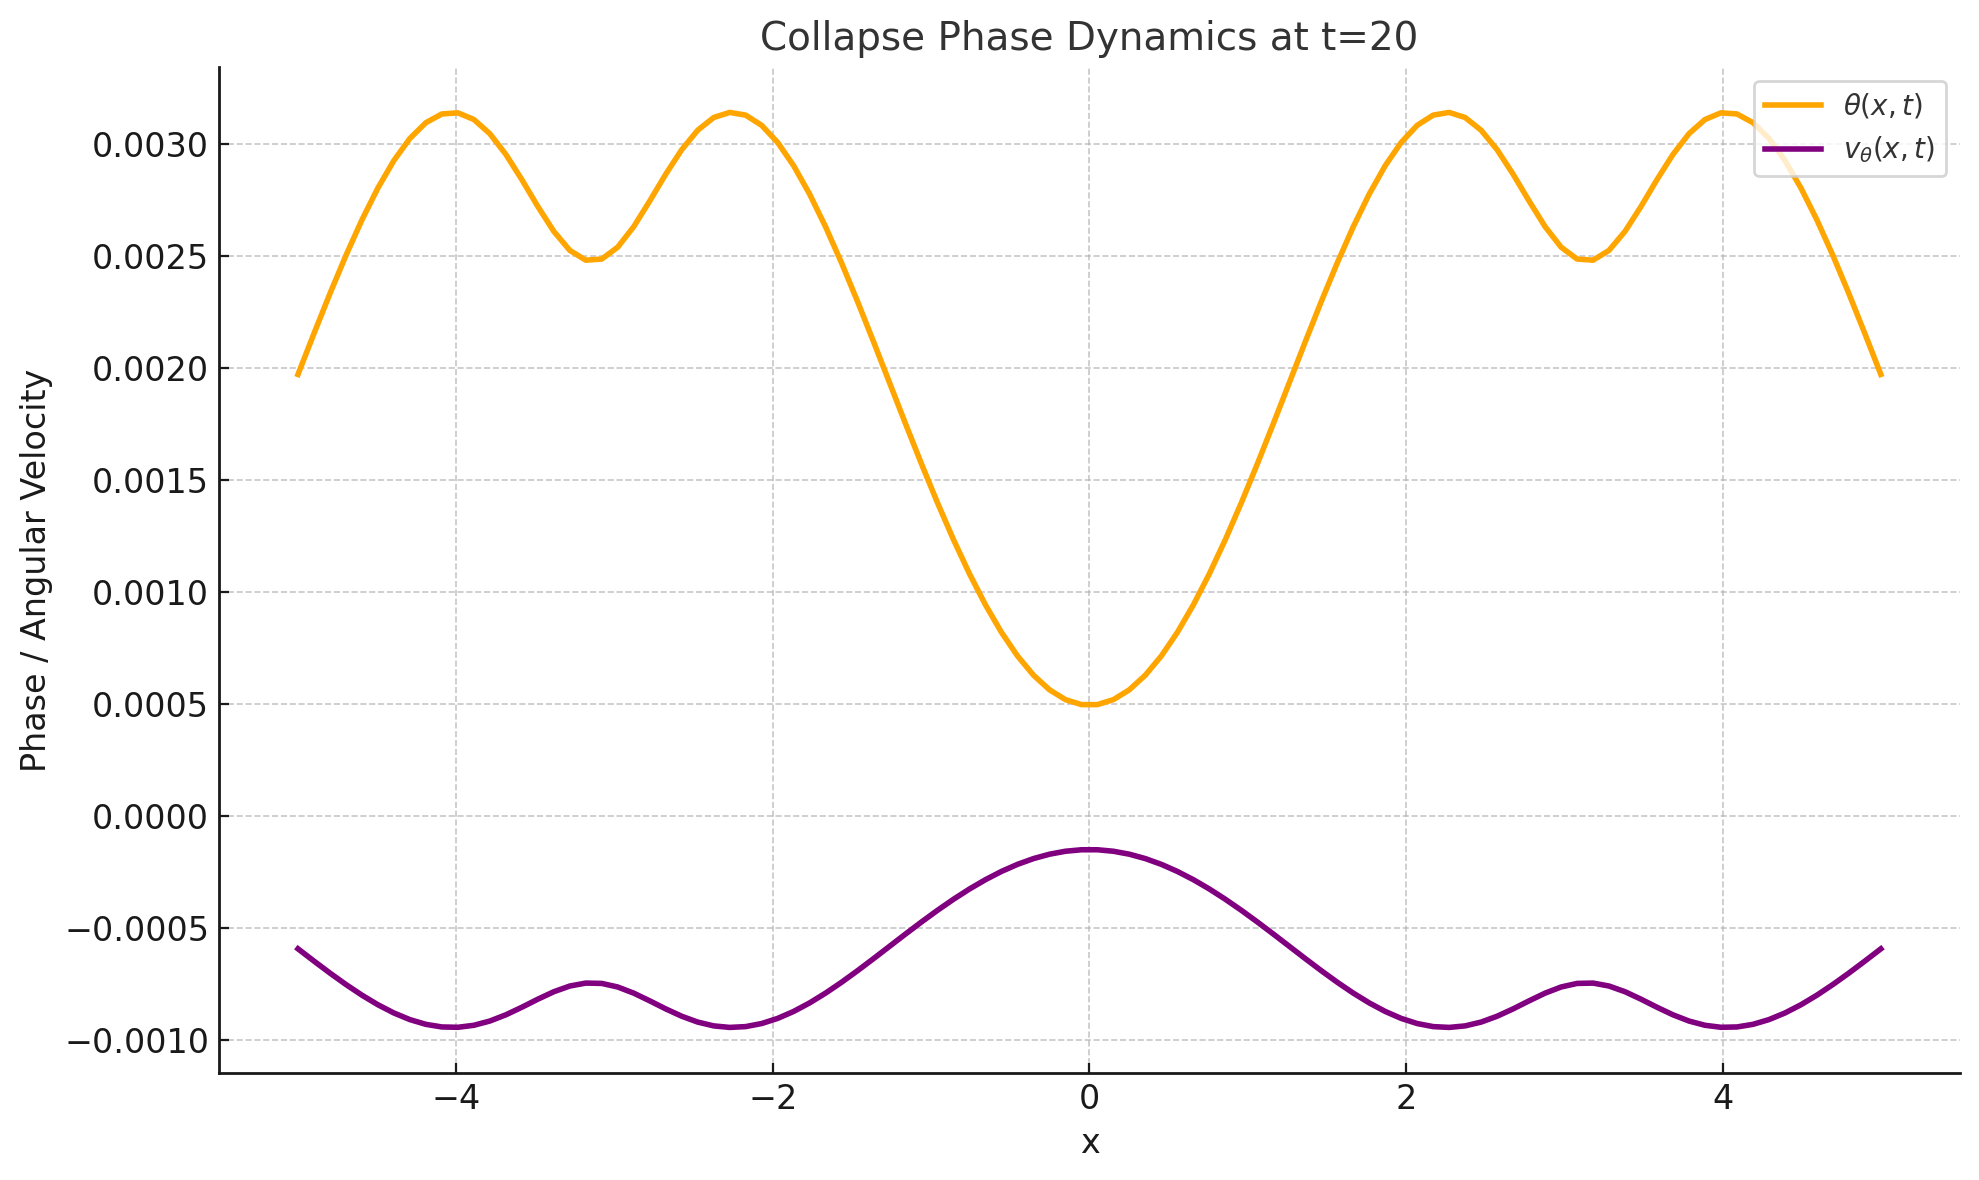
\includegraphics[width=\linewidth]{images/Collapse_phase.png}
    \caption{Simulation Plot showing Collapse Phase Angle.This captures the asymmetry and decay dynamics of the Measurement Field-where collapse rotation decelerates as the imaginary component drains out.}
\end{figure} \cite{chapter_time}


\nocite{*}
\printbibliography[title={Appendix B References}, keyword=chapter2]
